Five predictions were committed and pushed before any run
(\texttt{docs/predictions\_groundwater.md}): seeds 10--14, the full training budget,
v1's model families and settings, plus a 13-parameter \texttt{c\_mlp\_matched} for a
same-size classical comparison. The paper stated in advance that G-1 and G-2 were
expected to fail.

% Generated by scripts/report/paper_tables.py from results/adjudication_groundwater_v2.json.
\begin{table}[htbp]
  \centering
  \small
  \begin{tabular}{lr}
  \toprule
  Pre-registered claim, held on all five seeds & Measured \\
  \midrule
  Error below 1\% & 0.09\% \\
  Beats a classical network of the same size ($\ge1.3\times$) & 18.2$\times$ \\
  Beats the same circuit with random frequencies ($\ge1.5\times$) & 9.9$\times$ \\
  Gain over the MLP lies inside $\Omega$ ($\ge70\%$) & 99.4\% \\
  Waterlogged length within 5\% of the exact 713\,m & 714\,m \\
  \bottomrule
  \end{tabular}\\[8pt]
  \begin{tabular}{lrrr}
  \toprule
  Model & parameters & median error & waterlogged (m) \\
  \midrule
  SMCD circuit, 8 copies & 91 & 0.09\% & 714 \\
  same circuit, random frequencies & 91 & 0.92\% & 738 \\
  MLP, same size & 91 & 1.68\% & 672 \\
  frequency-matched classical, same size & 83 & 22.93\% & 0 \\
  MLP, large & 8{,}513 & 1.94\% & 707 \\
  \bottomrule
  \end{tabular}
  \caption{Groundwater, held-out seeds 10--14: the pre-registered claims for the SMCD
    circuit with eight copies (top) and every model's median relative $L^2$ error and
    waterlogged length (bottom). Exact waterlogged length: 713\,m.}
  \label{tab:gw}
\end{table}


\textbf{One of five confirmed} (Table~\ref{tab:gwv1}, Figure~\ref{fig:gwmodels}). The
SMCD circuit's improvement over \texttt{c\_mlp} lies almost entirely on its designed
frequencies (G-4), but the circuit does not solve the problem: its median water table
peaks near 4\,m instead of 8.5\,m, so it predicts no waterlogging at all. Unlike on the
heat equation, the same circuit with random frequencies does better here, and so does
a classical network with the same number of parameters (13), whose median error is
5.0\% and whose waterlogged length is 840\,m against the exact 713\,m. The
groundwater solution is dominated by a broad mound, not by the canal ripple, which is
what SMCD designs for; our reading is that on this problem the design's high
frequencies are a cost rather than a help.

\paragraph{With the v2 circuit: five of five confirmed.} The same five claims were
pre-registered for the v2 models of \S\ref{sec:followup}
(\texttt{docs/predictions\_v2.md}, pushed before any run;
\texttt{verify\_preregistration.py --v2}: 50 runs, 0 violations) and scored by the same
script (Table~\ref{tab:gwv2}, Figure~\ref{fig:gwmodelsv2}). The v2 circuit's median
error is 0.09\% (every seed below 0.5\%). It is 18$\times$ more accurate than a classical
network with the same 91 parameters and 9.9$\times$ more accurate than the same circuit
with random frequencies, on every paired seed; 99.4\% of its improvement over
\texttt{c\_mlp} lies inside $\Omega$; and its waterlogged length is 714\,m against the
exact 713\,m. Unlike on Poisson, the classical model handed the same frequencies does
not match it here (22.9\% error, no waterlogging predicted). A plausible reason, not
tested here, is that the solution's broad mound is poorly represented by a linear head
on those fixed sine features, while the circuit's trainable encoder can move its
frequencies. We read this as the strongest result in the
paper, with two limits: it is one problem, and the circuit is simulated, not run on
quantum hardware.

\begin{figure}[htbp]
  \centering
  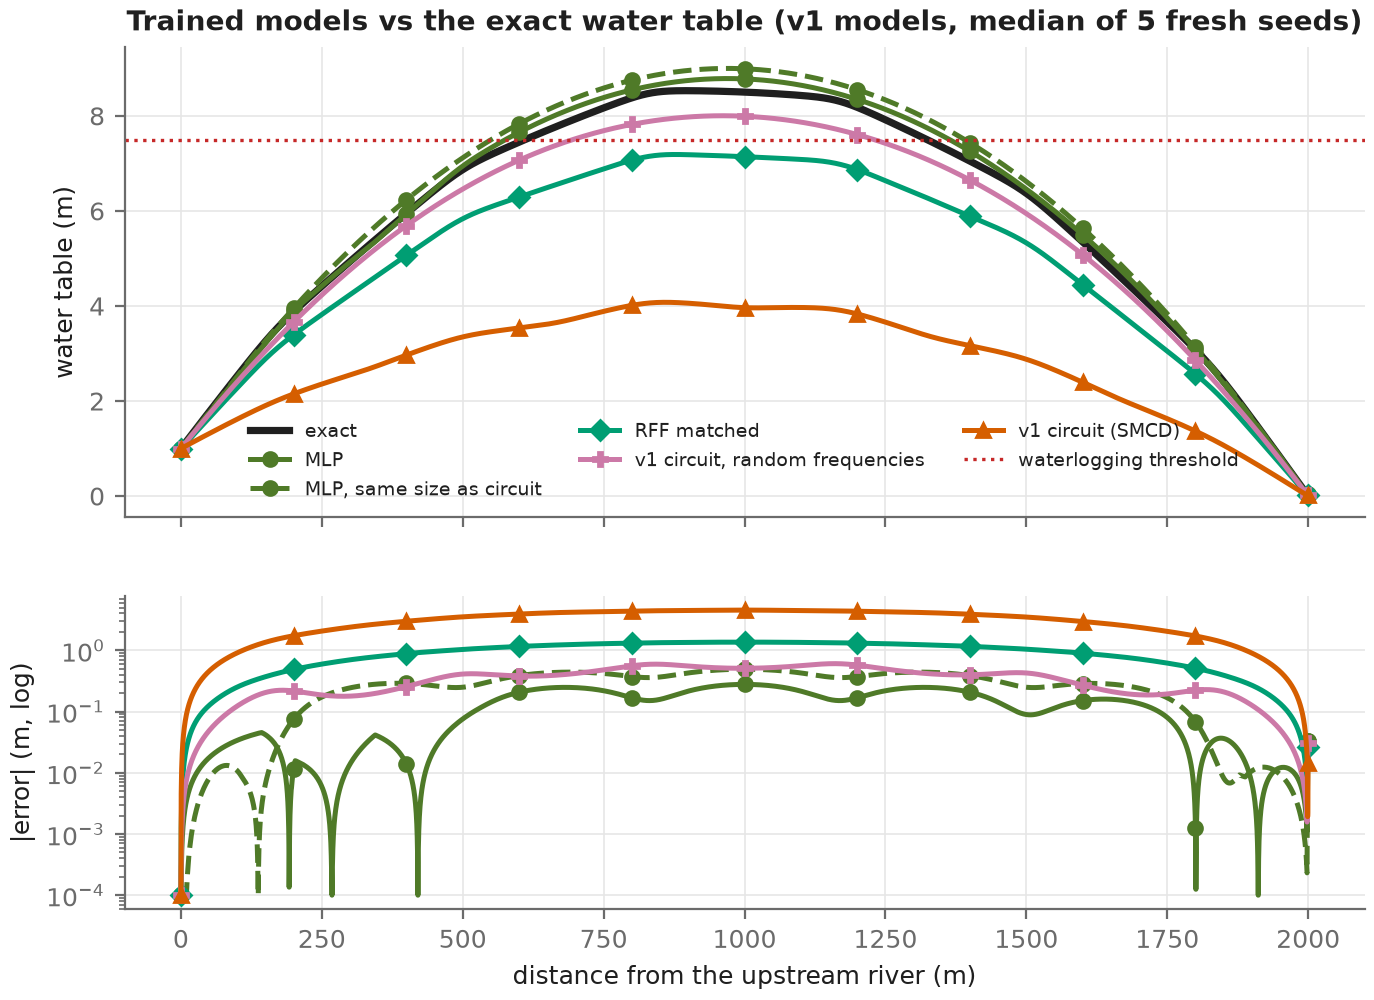
\includegraphics[width=0.85\linewidth]{../results/report/figures/groundwater_models_v1.png}
  \caption{Predicted water table of each trained model (median of seeds 10--14) against
    the exact solution. Dotted: the waterlogging threshold.}
  \label{fig:gwmodels}
\end{figure}

\begin{figure}[htbp]
  \centering
  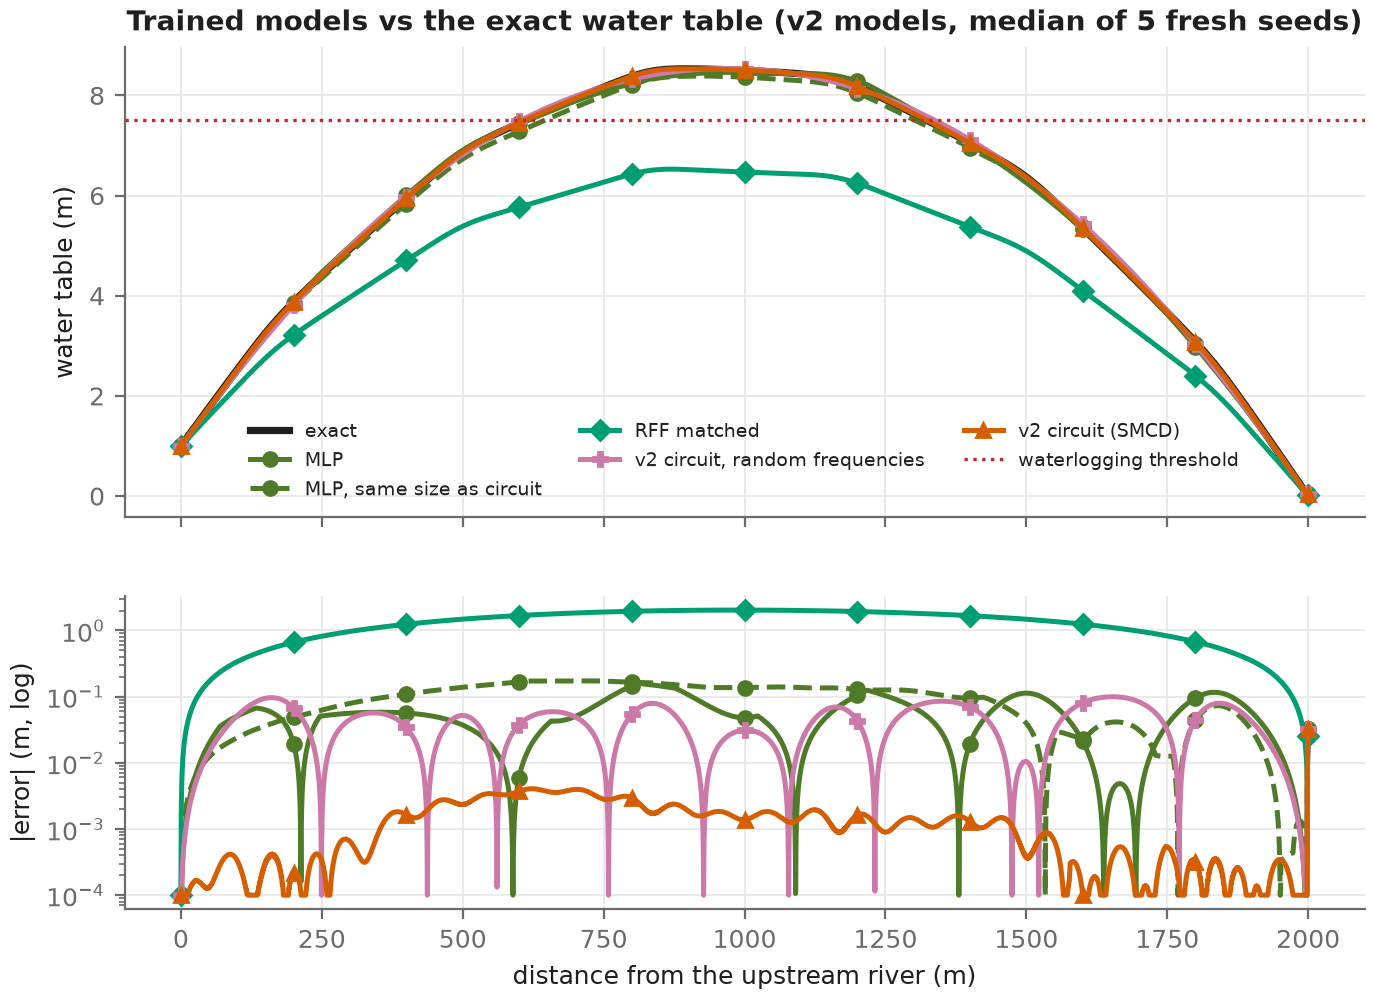
\includegraphics[width=0.85\linewidth]{../results/report/figures/groundwater_models_v2.png}
  \caption{The v2 models on the groundwater problem (median of seeds 10--14). Bottom: absolute
    error along the field; the v2 circuit stays within a few millimetres.}
  \label{fig:gwmodelsv2}
\end{figure}
